%%%%%%%%%%%%%%%%%%%%%%%%%%%%%%%%%%%%%%%%%%%%%%%%%%%%%%%
%%              Stochastic optimization              %%
%%%%%%%%%%%%%%%%%%%%%%%%%%%%%%%%%%%%%%%%%%%%%%%%%%%%%%%
\chapter{Managing uncertain requirements by means of stochastic optimization}
\chaptermark{Managing uncertain requirements by means of stochastic optimization}
\label{ch:stohasticopt}
%%%%%%%%%%%%%%%%%%%%%%%%%%%%%%%%%%%%%%%%%%%%%%%%%%%%%%%

This chapter explores the use of state-of-the-art stochastic optimization algorithms for managing uncertain requirements in design problems. We show how a set of design solutions can be obtained from the models defined in Chapter~\ref{ch:thermomechanical} via a stochastic version of \ac{MADS}, \texttt{StoMADS} \cite{Audet2019}. {\color{red}\texttt{StoMADS} returns a set of candidate solutions for a given stochastic programming problem which makes it an ideal choice for set-based design.}

The method described in this chapter can help simplify the algorithms introduced in Chapters \ref{ch:scalableSBD} and \ref{ch:TSEcont} by eliminating the steps involved in searching for a set of parametric optimal solutions.

%============================ METHODOLOGY ============================%
\section{Methodology} \label{sec:STOmethods}

Consider the optimization problem defined in Section \ref{subsec:SBDparametric} in Equation~(\ref{eq:SBDoptproblem}). The objectives and constraints are a function of uncertain parameters $\mathbf{p}$. In this section we denote the uncertain parameters by random variables $\mathbf{P} = \left[P_1,P_2,\cdots,P_m\right]$ (not to be confused with the reliability vector defined in Chapter~\ref{ch:TSEcont}). The objective and constraints functions in Equation~(\ref{eq:SBDoptproblem}) are deterministic in nature. By replacing the uncertain parameters with their random counterparts, the objective and constraint functions become stochastic

\begin{equation}
	\begin{aligned}
		& \underset{\mathbf{x}}{\text{minimize}}
		& & \hat{f}(\mathbf{x})~\textrm{where}~\hat{f}(\mathbf{x})=\mathbb{E}_{\mathbf{P}}\left[\hat{f}_{\mathbf{P}}(\mathbf{x})\right]\\
		& \text{subject to}
		& & \hat{\mathbf{g}}(\mathbf{x}) \le \mathbf{0}~\textrm{where}~\hat{\mathbf{g}}(\mathbf{x})=\mathbb{E}_{\mathbf{P}}\left[\hat{\mathbf{g}}_{\mathbf{P}}(\mathbf{x})\right],
	\end{aligned}
	\label{eq:STOoptproblem}
\end{equation}
%
where $\mathbb{E}_{\mathbf{P}}$ denotes the expectation with respect to the vector of random variables $\mathbf{P}$. $\hat{f}_{\mathbf{P}}(\mathbf{x})$ and $\hat{\mathbf{g}}_{\mathbf{P}}(\mathbf{x})$ denote the stochastic version of the surrogate models for the engineering design problem being solved.

$\hat{f}_{\mathbf{P}}(\mathbf{x})$ and $\hat{\mathbf{g}}_{\mathbf{P}}(\mathbf{x})$ are obtained from their deterministic counterparts $\hat{f}(\mathbf{x};{\mathbf{p}})$ and $\hat{\mathbf{g}}(\mathbf{x};{\mathbf{p}})$ by randomly sampling the components of the parameters vector $\mathbf{p}$ from a joint \ac{PDF} $F_{\mathbf{X}}(\mathbf{p})$. In this chapter, we use a uniform distribution for the joint \ac{PDF} although other distributions can be used depending on the problem.

The optimization problem in Equation~(\ref{eq:STOoptproblem}) is solved via \texttt{StoMADS} to obtain a set of candidate solutions for the optimizer $\mathbf{X}^*=  \{ \mathbf{x}^*_1,\mathbf{x}^*_2,\ldots,\mathbf{x}^*_w \} $.

We demonstrate the capabilities of \texttt{StoMADS} by solving a \ac{TRS} remanufacturing problem where uncertain parameters are involved.

%========================= APPLICATION PROBLEM =======================%
\section{Application problem} \label{sec:STOcasestudy}

We investigate the deposition of a circumferential stiffener on the outer casing of a \ac{TRS} (shown in Figure~\ref{fig:TRSoverview}) subject to 4 uncertain temperature loads (shown in Figure~\ref{fig:thermalloads}). We formulate the problem as follows:
%
\begin{equation} \label{eq:Stoproblemdet}
    \begin{aligned}
        & \underset{\mathbf{x}}{\text{minimize}}
        & & \hat{f}(\mathbf{x};\mathbf{p}) = -\hat{n_{\textrm{safety}}}(\mathbf{x};T_1,T_2,T_3,T_4)\\
        & \text{subject to}
        & & {g_{\textrm{linear}}}(\mathbf{x}) = x_3 + x_1 - W_{\textrm{total}} \le 0,\\
    \end{aligned}
\end{equation}
%
where $\mathbf{x} = \left[x_1,x_2,x_3\right]^{\mathrm{T}}$. The objective function is obtained from a surrogate model for the safety factor $\hat{n_{\textrm{safety}}}(\mathbf{x};\mathbf{p})$, where the inputs are the stiffener dimensions $x_1,x_2,$ and $x_3$ and temperature loads $T_1,T_2,T_3,$ and $T_4$.

The design variables for this problem govern the circumferential stiffener geometry (given by $x_1,x_2,$ and $x_3$). The uncertain parameters for this problem are the 4 temperature loads experienced by the \ac{TRS} ($T_1,T_2,T_3,$ and $T_4$). We extract the relevant design variables and parameters from Table~\ref{table:modelinputs} and list them in the tables below.


\begin{table}[h!]
    \centering
    \renewcommand{\arraystretch}{1.0}% Wider
    \small\addtolength{\tabcolsep}{-2pt}
    \caption{Design variables ${\textbf{x}}$}
    \label{table:STOmodelinputs}
    \begin{tabular}{lcccc}
    \hline\hline
    \bf Design variable & \bf Notation & \bf Units & \bf Lower bound & \bf Upper bound \\
    \hline
    Stiffener axial position & $x_1$ & mm & 37 & 145 \\
    Stiffener thickness  & $x_2$ & mm & 2 & 10 \\
    Stiffener width & $x_3$ & mm & 10 & 40  \\
    \hline\hline
    \end{tabular}
\end{table}

\begin{table}[h!]
	\centering
	\renewcommand{\arraystretch}{1.0}% Wider
	\small\addtolength{\tabcolsep}{-2pt}
	\caption{Relevant model parameters and constants}
	\label{table:STOmodelparameters}
	\begin{tabular}{lccc}
	\hline\hline
	\bf Parameter/constant & \bf Notation & \bf Units & \bf Value \\
	\hline
    %================================================================
    \multicolumn{4}{c}{Uncertain parameters $\mathbf{p}$} \\ 
	Nacelle temperature & $T_1$ & $^{o}$C & $300 \pm 100$ \\ 
	Tailcone temperature & $T_2$ & $^{o}$C & $400 \pm 100$ \\ 
	Rotor temperature & $T_3$ & $^{o}$C & $450 \pm 100$ \\ 
	Gas surface temperature & $T_4$ & $^{o}$C & $600 \pm 100$ \\ \hline
    %================================================================
    \multicolumn{4}{c}{Constant parameters} \\
	Laser Power & ${P_\textrm{laser}}$ & W &  3806 \\ 
	Laser beam radius & ${r_l}$ & mm & 14.2 \\ 
	Scanning speed& ${V}$ & mm/s & 5.0 \\ 
	Laser penetration depth & $D_p$ & mm & 5.0 \\
	Substrate base width & $W_{\textrm{total}}$ & mm & $155$ \\
	%================================================================
	\hline\hline
	\end{tabular}
\end{table}

The design problem in Equation~(\ref{eq:Stoproblemdet}) is transformed to its stochastic counterpart by randomly sampling the uncertain parameters from a uniform distribution
%
\begin{equation}
	\begin{aligned}
		& \underset{\mathbf{x}}{\text{minimize}}
		& & \mathbb{E}_{\mathbf{P}}\left[\hat{f}_{\mathbf{P}}(\mathbf{x})\right]\\
		& \text{subject to}
		& & {g_{\textrm{linear}}}(\mathbf{x}) = x_3 + x_1 - W_{\textrm{total}} \le 0,\\
	\end{aligned}
	\label{eq:STOproblemsto}
\end{equation}
%
where $\mathbf{x} = \left[x_1,x_2,x_3\right]^{\textrm{T}}$, $\mathbf{P} = \left[T_1,T_2,T_3,T_4\right]^{\textrm{T}}$, and $\hat{f}_{\mathbf{P}}(\mathbf{x})$ is the stochastic version of the objective. The random vector $\mathbf{P}$ has its components sampled from a uniform distribution. The constraint remains unchanged since its does not involve uncertain parameters.

Before solving the problem in Equation~(\ref{eq:STOproblemsto}), we perform Monte Carlo simulation on the stochastic objective function to determine the effect of the design variables on the expected value of the objective.

%---------------------------------------------------------------------%
% Monte Carlo simulation
\subsection{Monte Carlo simulation of stochastic objective function} \label{subsec:MCSsto}


For each design variable in $\mathbf{x}$, we vary one variable at a time while holding the others fixed at their nominal values as given by Table~\ref{table:STOmodelinputs}. The stochastic objective function is called $1000$ times for a given combination of variables while randomly sampling the design parameters in $\mathbf{P}$ from a uniform distribution. The upper and lower bound for the uniform distribution that each random parameter $P_m$ follows is given by Table~\ref{table:STOmodelparameters}.

The results of the Monte Carlo simulation are visualized in Figure~\ref{fig:MSCStoblackbox}. From these results, it can be seen that the expectation of the stochastic objective function $\mathbb{E}_{\mathbf{P}}\left[\hat{f}_{\mathbf{P}}(\mathbf{x})\right]$ as given by the mean of the 1000 samples for each run is dependant on the variables in $\mathbf{x}$. It can be seen that $\mathbb{E}_{\mathbf{P}}\left[\hat{f}_{\mathbf{P}}(\mathbf{x})\right]$ is maximized in the range $ 72.5 \le x_1 \le 100 $ and at $x_2 \approx 15$ and $x_3 \approx 87.5$.

\begin{figure}[h!]
	\centering
	\subfloat[Effect of $x1$, $x2=6$ mm, $x_3=25$ mm\label{fig:X1sweep}]{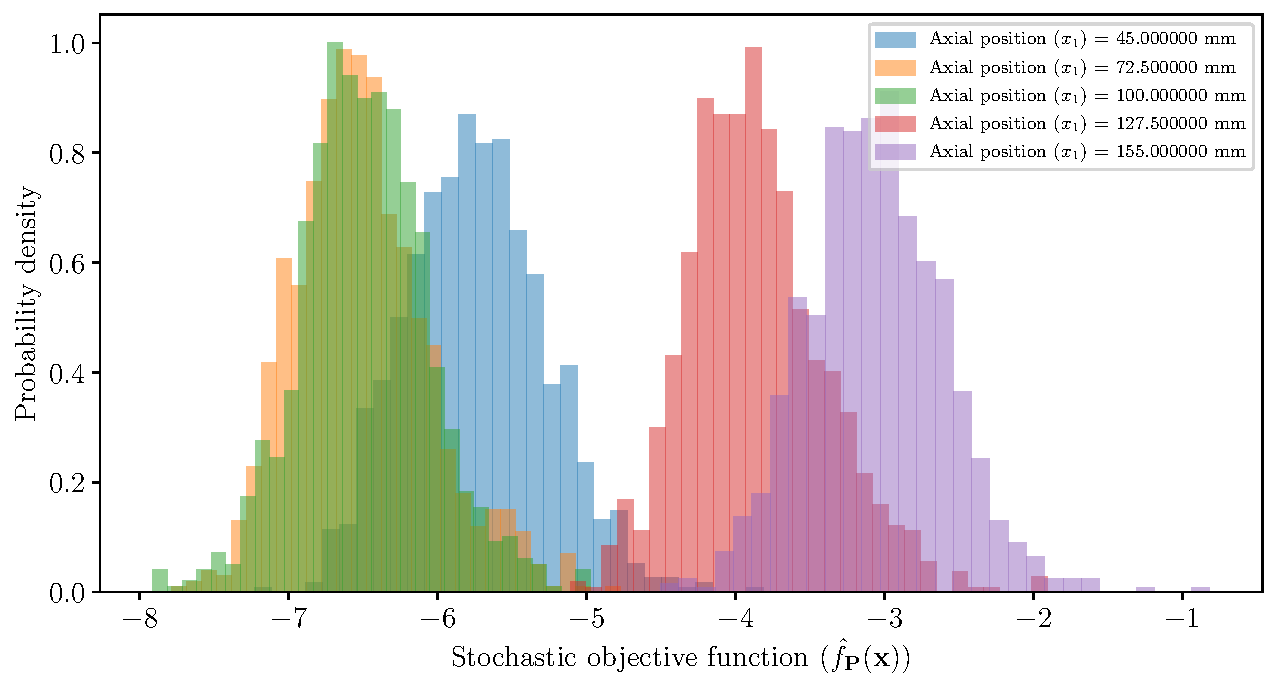
\includegraphics[width=0.9\textwidth]{PDF_nsafety_X1}} 
	
	\subfloat[Effect of $x2$, $x1=91$ mm, $x_3=25$ mm\label{fig:X2sweep}]{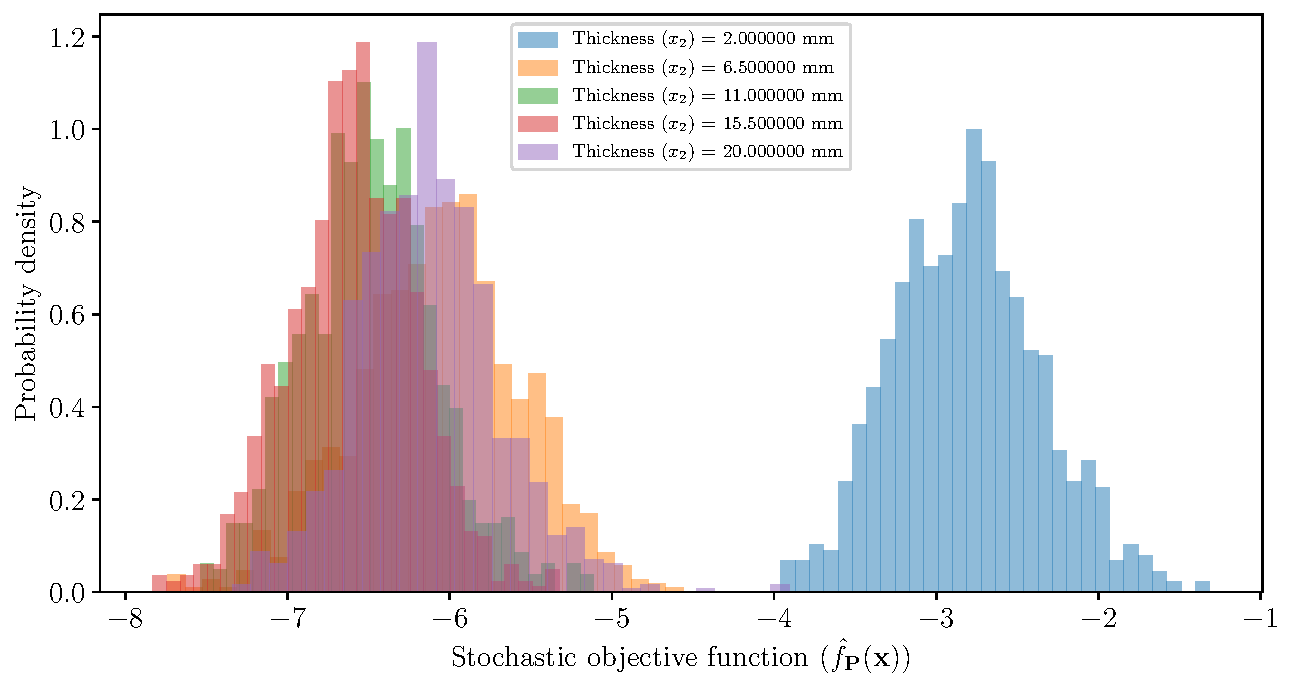
\includegraphics[width=0.9\textwidth]{PDF_nsafety_X2}} 
	\caption[]{Monte Carlo simulation of $\hat{f}_{\mathbf{P}}(\mathbf{x})$ using $1000$ samples}
\end{figure}

\begin{figure}[h!]
	\ContinuedFloat % split subfigure across multiple pages
	\subfloat[Effect of $x3$, $x1=91$ mm, $x_2=6$ mm\label{fig:X3sweep}]{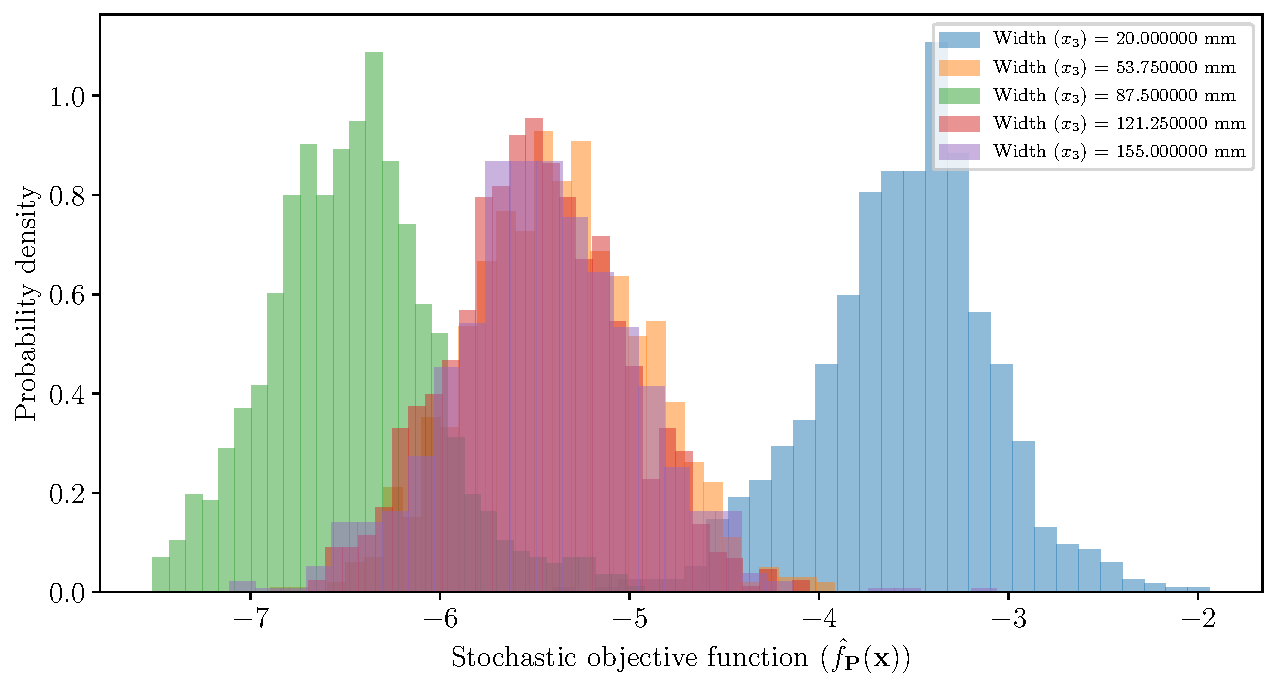
\includegraphics[width=0.9\textwidth]{PDF_nsafety_X3}} 
	\caption[Monte Carlo simulation of $\hat{f}_{\mathbf{P}}(\mathbf{x})$ using $1000$ samples]{Monte Carlo simulation of $\hat{f}_{\mathbf{P}}(\mathbf{x})$ using $1000$ samples \emph{(cont.)}}
	\label{fig:MSCStoblackbox}
\end{figure}

%---------------------------------------------------------------------%
% Monte Carlo simulation
\subsection{\texttt{StoMADS} results for stochastic optimization problem} \label{subsec:STOMADSresults}

We solved the problem in Equation~(\ref{eq:STOproblemsto}) using \texttt{StoMADS-PB} to obtain a set of solutions. This algorithm is a version of \texttt{StoMADS} where constraints are handled by the progressive barrier approach \cite{Audet2009}.

The problem is also solved using the deterministic version of the algorithm \texttt{NOMAD} in order to be used as a benchmark for the quality of the solutions obtained via \texttt{StoMADS-PB} \cite{LeDigabel2011}. 

It is recommended by the developers of \texttt{StoMADS-PB} to set the maximum number of blackbox evaluations parameter of the algorithm to \texttt{max\_bb\_eval}$ = (n+1) \times 1000$, where $n$ is the number of variables. As a result, 4000 iterations where used with \texttt{StoMADS-PB}.

The best four solutions in terms of the expectation of the objective function are listed in Table~\ref{table:StoMADSresults}. In order to compute the expectation, a Monte Carlo simulation was performed for each of the solutions obtained in Table~\ref{table:StoMADSresults}. The results of the Monte Carlo simulation are shown in Figure~\ref{fig:MCSstomadsresults}.

\begin{figure}[h!]
	\centering
	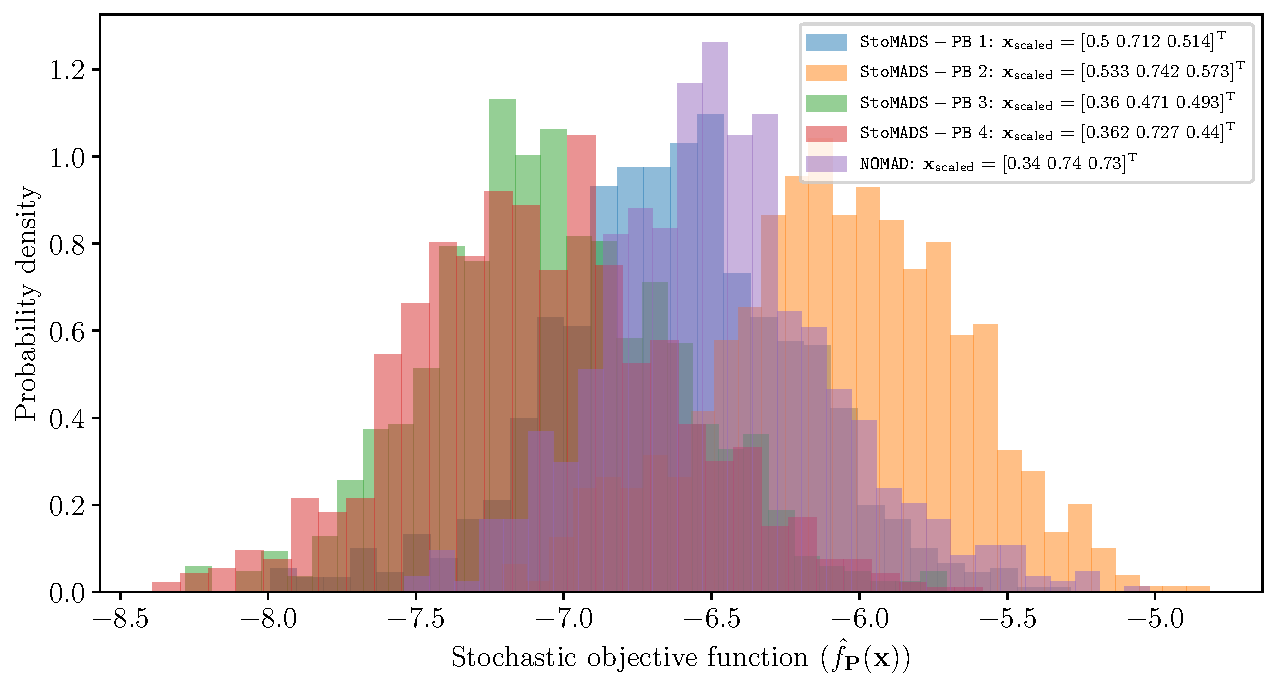
\includegraphics[width=0.8\textwidth]{PDF_nsafety_soln.pdf}
	\caption{Monte Carlo simulation results of \texttt{StoMADS-PB} and \texttt{NOMAD} solutions}
	\label{fig:MCSstomadsresults}
\end{figure}

\renewcommand{\ocwa}{1.5cm} % index column width
\renewcommand{\ocwb}{1.85cm} % decision arc column width
\renewcommand{\ocwc}{1.85cm} % objective column width
\renewcommand{\ocwd}{1.85cm} % constraints column width
\renewcommand{\ocwe}{1.85cm} % design arc column width
\newcommand{\ocwf}{1.85cm} % design arc column width
\newcommand{\ocwg}{1.85cm} % design arc column width

\begin{table}[h!]
	\centering
	\renewcommand{\arraystretch}{1.0}% Wider
	\addtolength{\tabcolsep}{-2pt}
	\caption{\ac{TRS} optimization problem results}
	\label{table:StoMADSresults}
	\begin{tabular}{>{\centering\arraybackslash}p{\ocwa}|>{\centering\arraybackslash}p{\ocwb}>{\centering\arraybackslash}p{\ocwc}>{\centering\arraybackslash}p{\ocwd}|>{\centering\arraybackslash}p{\ocwe}>{\centering\arraybackslash}p{\ocwf}|>{\centering\arraybackslash}p{\ocwg}}
	\hline\hline
	\bf Solution No. & \bf Axial Position & \bf Thickness & \bf Width & \multicolumn{2}{c|}{\bf Objective} & \bf Constraint \\ 
	 & \multirow{2}{\ocwb}{\centering $x_1$} & \multirow{2}{\ocwc}{\centering $x_2$} & \multirow{2}{\ocwd}{\centering $x_3$} & \multicolumn{2}{c|}{$\hat{f}_{\mathbf{P}}(\mathbf{x})$} & \multirow{2}{\ocwg}{\centering $g_{\mathrm{linear}}(\mathbf{x})$} \\ 
	 & & & & Expectation $\mathbb{E}_{\mathbf{P}}\left[\hat{f}_{\mathbf{P}}(\mathbf{x})\right]$ & Variance $\sigma^2$ & \\ \hline
	%================================================================
	\multicolumn{7}{c}{Algorithm: \texttt{StoMADS-PB} } \\\hline
	%================================================================
	1 & 100.0 & 14.8 & 89.4 & -6.63 & 0.417 & -11.58 \\
	%================================================================
	2 & 103.6 & 15.4 & 97.4 & -6.07 & 0.417 & -0.0004 \\
	%================================================================
	3 & 84.6 & 10.5 & 86.5 & -7.03 & 0.415 & -29.9 \\
	%================================================================
	4 & 84.8 & 15.1 & 79.4 & -7.08 & 0.447 & -36.8 \\\hline
	%================================================================
	\multicolumn{7}{c}{Algorithm: \texttt{NOMAD} } \\\hline
	%================================================================
	1 & 82.4 & 15.3 & 118.6 & -6.48 & 0.389 & -0.05 \\
	%================================================================
	\hline\hline
	\end{tabular}
\end{table}

It can be seen from Table~\ref{table:StoMADSresults} that the \texttt{StoMADS-PB} algorithm performs better than the \texttt{NOMAD} algorithm when comparing the expected value of the objective function at the optimizer. Only \texttt{StoMADS-PB} candidate solution 2 underperformed in terms of the expectation of the objective function relative to the \texttt{NOMAD} solution. Furthermore it can be seen that the constraint was inactive for the best performing candidate solution. It should also be noted that although the \texttt{NOMAD} algorithm is deterministic, running the problem with the same initial conditions and algorithm parameters will yield a variety of solutions due to the stochastic nature of the objective function.

We will now summarize the implications of this approach for obtaining set-based solutions in relation to the set-based design approaches that have been developed in this thesis.

%============================== SUMMARY ================================%
\section{Summary}
\label{sec:stohasticoptsummary}

This chapter presented an alternative strategy for solving parametric optimization problems. Rather than sampling the parameter space and solving the optimization problem for a given sample of parameter values, \texttt{StomMADS} can be used to directly obtain a set of solutions with an equivalent stochastic objective and constraint functions where the parameters are sampled from their respective random distributions.

The approach presented in this chapter can be used to improve Algorithms~\ref{algo:PODalgo} and \ref{algo:SBDOptalgo}. Solving the problem in Equation~(\ref{eq:STOoptproblem}) can substitute steps 1 through 8 in Algorithm~\ref{algo:PODalgo}. However, the solution to the problem in Equation~(\ref{eq:STOoptproblem}) only outputs the optimizer values in the design space. Corresponding parameter values cannot be obtained since they are intrinsic to the stochastic version of the objective and constraint functions. The set of optimizers and their corresponding parameter values are needed by Algorithm~\ref{algo:PODalgo} to construct a response surface in the parameter space.

However, the approach in this chapter can substitute steps 3 through 5 within Algorithm \ref{algo:SBDOptalgo} by randomly selecting requirement arcs from $\Omega_R$ in the stochastic version of the problem. The requirement arc corresponding to each solution in $S_{E}^*$ is not needed since only the frequency of the design arcs is needed to isolate the set-based solution. However, the development version of \texttt{StoMADS} is restricted to optimization problems with continous variables and needs to be further developed to include mixed variable programming problems such as those in Chapter~\ref{ch:TSEcont}.

The approach presented in this chapter can prove useful to designers who are accustomed to more traditional design practices involving point-based design. This is because \texttt{StoMADS} has a similar interface to most available deterministic design optimization approaches that output a single design solution.